\documentclass{article}

% Pakete
\usepackage[utf8]{inputenc}
\usepackage[ngerman]{babel}
\usepackage{amsmath}
\usepackage{graphicx}
\usepackage{float}
\usepackage{cite}
\usepackage{multirow}
\usepackage{booktabs}


% Titel und Autor
\title{RNA Analytik}
\author{Thorsten Enge \and David Maruhn}
\date{\today}

\begin{document}

% Titel erstellen
\maketitle

% Inhaltsverzeichnis
\tableofcontents
\newpage

% Einleitung
\section{Einleitung}

Das Ziel der RNA-Analytik mittels qPCR ist einerseits die Quantifizierung von RNA, andererseits können Single Nucleotide Polymorphisms (SNPs) detektiert werden. Hierfür muss zuerst die RNA isoliert werden, um sie anschließend in cDNA umzuschreiben. Die cDNA wird während der qPCR amplifiziert. Ein Farbstoff, der bei Bindung an doppelsträngige DNA seine Fluoreszenz ändert, dient dazu, die Menge an RNA in der Probe zu bestimmen. Anschließend wird eine Schmelzkurvenanalyse durchgeführt, bei der während eines finalen Denaturierungsschrittes die Fluoreszenz gemessen wird. Während bei der DNA-Analytik untersucht wird, ob eine bestimmte DNA-Sequenz im Genom vorhanden ist, wird bei der RNA-Analytik untersucht, ob und wie stark ein bestimmtes Gen transkribiert wird. Das Vorhandensein eines Gens im Genom bedeutet nicht zwangsläufig, dass dieses Gen auch transkribiert wird. Mechanismen wie DNA-Methylierung, Histonmodifikation, Transkriptionsfaktoren und Enhancer bzw. Silencer beeinflussen die Transkription eines Gens. Durch die Analyse der RNA kann einerseits das Vorhandensein eines Gens im Genom bestätigt werden, andererseits kann durch die Quantifizierung Rückschlüsse auf die Transkriptionsrate und somit auf die Aktivität des Gens gezogen werden. Das Nichtvorhandensein eines Transkripts bedeutet entweder das Fehlen des Gens im Genom oder eine sehr geringe Transkriptionsrate.

% Materialien und Methoden
\section{Materialien und Methoden}

Es werden zwei unterschiedliche immortalisierte humane Zellkulturen analysiert, die Durchführung unterscheidet sich nicht zwischen den beiden Zellkulturen.

\subsection*{Thermocycler LightCycler 96}
Der LightCycler von Roche ist ein Thermocycler mit echtzeit Flouroszensmessung. Er dient zur Durchführung der qPCR. Die zugehörige Software ermöglicht die Auswertung der Messdaten.

\subsection*{Spektrophotometer \mbox{DS-11+ -DeNovix}}
Das Spektrophotometer dient zur Bestimmung der Konzentration und Reinheit der RNA. Es ermöglicht die Messung von Absorption und Fluoreszenz.

\subsection*{Monarch Total RNA Miniprep Kit}
Das Kit dient zur Isolierung von RNA aus Zellen. Es enthält alle notwendigen Reagenzien und Materialien.
\begin{figure}[H]
    \centering
    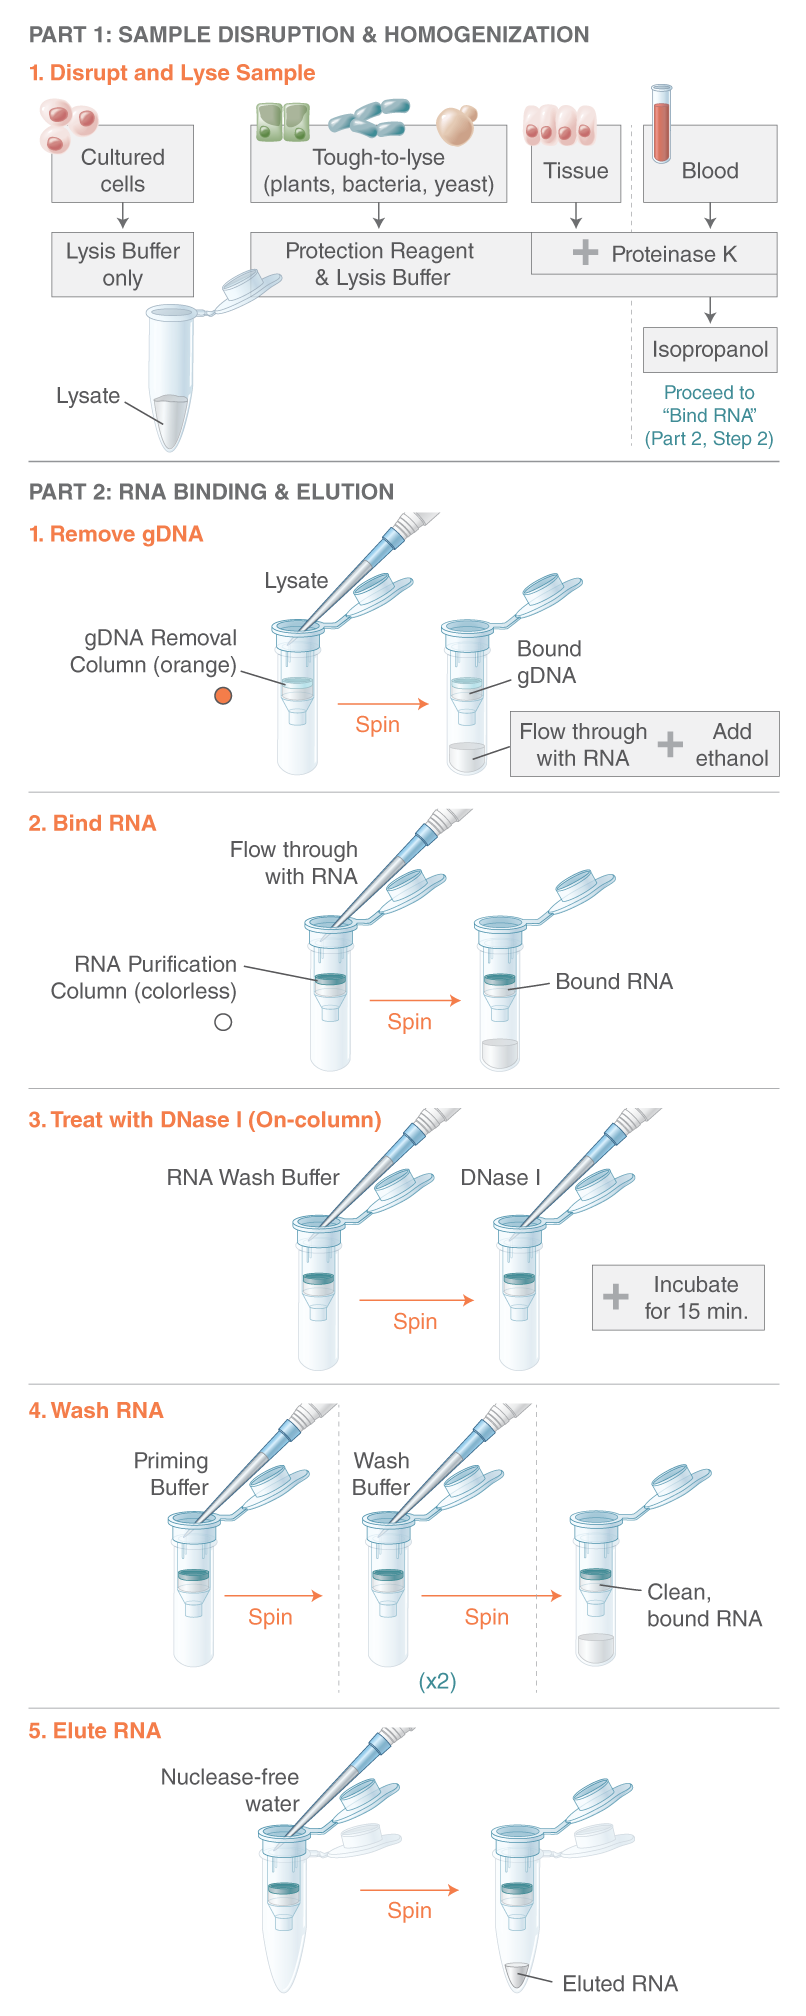
\includegraphics[height=\textheight]{images/monarch.png}
    \caption{Monarch Total RNA Miniprep Kit}
    \label{fig:monarch}
\end{figure}



\begin{itemize}
    \item \textbf{Monarch gDNA Removal Columns}: Diese Säulen dienen zur Entfernung genomischer DNA aus der Probe, um eine reine RNA-Fraktion zu erhalten.
    \item \textbf{Monarch RNA Purification Columns}: Diese Säulen werden zur Bindung und Reinigung der RNA verwendet.
    \item \textbf{Monarch Spin Collection Tubes}: Diese Röhrchen werden für die Zentrifugation und Sammlung der durch die Säulen fließenden Lösungen verwendet.
    \item \textbf{Monarch DNA/RNA Protection Reagent (2X)}: Ein Reagenz zur Stabilisierung und Schutz der DNA und RNA während der Probenvorbereitung und Lagerung.
    \item \textbf{Monarch RNA Lysis Buffer}: Ein Puffer, der die Zellen lysiert und die RNA für die Bindung an die Reinigungssäule vorbereitet.
    \item \textbf{Monarch Proteinase K (lyophilisiert)}: Ein Enzym, das Proteine in der Probe abbaut und somit die Reinheit der isolierten RNA verbessert.
    \item \textbf{Monarch Proteinase K Resuspension Buffer}: Ein Puffer zur Wiederaufbereitung der lyophilisierten Proteinase K.
    \item \textbf{Monarch Proteinase K Reaction Buffer}: Ein Puffer, der die optimale Aktivität der Proteinase K während der Inkubation gewährleistet.
    \item \textbf{Monarch DNase I (lyophilisiert)}: Ein Enzym zur Verdauung und Entfernung von genomischer DNA, um eine kontaminationsfreie RNA-Isolierung zu gewährleisten.
    \item \textbf{Monarch DNase I Reaction Buffer}: Ein Puffer, der die optimale Aktivität der DNase I während der DNA-Verdauung gewährleistet.
    \item \textbf{Monarch RNA Priming Buffer}: Ein Puffer, der die RNA für die endgültige Reinigung und Elution vorbereitet.
    \item \textbf{Monarch RNA Wash Buffer (5X)}: Ein konzentrierter Waschpuffer zur Entfernung von Verunreinigungen während der RNA-Reinigung.
\end{itemize}


\section{Durchführung}



\section{Ergebnisse}


% Diskussion
\section{Diskussion}

% Schlussfolgerung
\section{Schlussfolgerung}

% Literaturverzeichnis
\bibliographystyle{plain}
\bibliography{literatur}

\end{document}
